% Joshua Reed
% Fall, 2017
% 
% Homework for random processes.

% chktex-file 1 chktex-file 13 chktex-file 25 chktex-file 3 chktex-file 36

\documentclass[12pt]{article}
\usepackage[margin=1in]{geometry} 
\usepackage{amsmath,amsthm,amssymb}
\usepackage{listings}
\usepackage[compact]{titlesec}
\usepackage{graphicx}
\usepackage{listings}
\usepackage{commath}
\usepackage{enumitem}
\usepackage{tikz}
\usepackage{float}
\usetikzlibrary{shapes,arrows,positioning}
\graphicspath{{img/}}

\setlength\parindent{00pt}
\setlength{\parskip}{\baselineskip}
\titlespacing{\section}{0pt}{5pt}{-\parskip}
\titlespacing{\subsection}{0pt}{-5pt}{-\parskip}
\titlespacing{\subsubsection}{0pt}{-8pt}{-\parskip}

\makeatletter
\newcommand{\vx}{\vec{x}\@ifnextchar{^}{\,}{}}
\newcommand{\vy}{\vec{y}\@ifnextchar{^}{\,}{}}
\newcommand{\vX}{\vec{X}\@ifnextchar{^}{\,}{}}
\newcommand{\vY}{\vec{Y}\@ifnextchar{^}{\,}{}}
\makeatother

\newcommand*\Eval[3]{\left.#1\right\rvert_{#2}^{#3}}


\makeatletter
\renewcommand{\@seccntformat}[1]{}
\makeatother

% The below is for creating block diagrams...
\tikzset{block/.style={draw, 
                       rectangle, 
                       minimum height=3em, 
                       minimum width=6em},
         input/.style={coordinate}}

\begin{document}

{%Header section
  \large \bfseries 
  Joshua Reed\\
  Fall, 2017

  \begin{center}
    {\huge Homework for Chapter 8}

    EE 520 - Random Processes \\% chktex 8 
  \normalsize Problems: 8.1, 8.22, 8.40, 8.44, and 8.51
  \end{center}}
 
 
\section{8.21} 
\subsection{Exercise}
Given a random sequence $X[n]$ for $n \geq0$ with conditional pdfs
\begin{align*}
  f_X(x_n|x_{n-1})&=\alpha e^{-\alpha(x_n-x_{n-1})}u(x_n-x_{n-1})\text{,  for } n\geq 1,
\end{align*}
with $u(x)$ the unit-step function and the intitial pdf $f_X(x_0)=\delta(x_0)$. Take $\alpha > 0$.
\begin{enumerate}[label=(\alph*)]
  \item Find the first-order pdf $f_X(x_n)$ for $n=2$.

The integration of $dx_0$ below comes from.
\begin{align*}
 f(x_0) &= \delta(x_0)\big|_{x_0=0} \\
  &= 1
\end{align*}
Building up from the known first-order pdf of $x_0$.
\begin{align*}
 f(x_0,x_1,x_2) &= fx(x_0)f_X(x_1|x_0)f_X(x_2|x_1) \\
\end{align*}
And then removing the reliance upon $x_0$ and $x_1$ via integration.
\begin{align*}
 f(x_2)         &= \int \int fx(x_0)f_X(x_1|x_0)f_X(x_2|x_1)\ dx_0\ dx_1 \\
                &= \int \int \delta(x_0) f_X(x_1|x_0)f_X(x_2|x_1)\ dx_0\ dx_1 \\
                &= \int f_X(x_1|x_0 = 0)f_X(x_2|x_1)\ dx_1 \text{, \qquad    here $\int \delta(x)f(x) dx = f(0)$}\\
                &= \int \alpha e^{-\alpha(x_1-0)}u(x_1)\alpha e^{-\alpha(x_2-x_1)}u(x_2-x_1)\ dx_1 \\
                &= \alpha^2\int e^{-\alpha(x_1+x_2-x_1)}u(x_1)u(x_2-x_1)\ dx_1 \\
                &= \alpha^2\int e^{-\alpha x_2}u(x_1)u(x_2-x_1)\ dx_1 \\
                &= \alpha^2\int^0_{-\infty} e^{-\alpha x_2}u(x_2-x_1)\ dx_1 \\
                &= \alpha^2\left[e^{-\alpha x_2}ramp(x_2-x_1)\ \big|^0_{-\infty}\right] \text{, \qquad where $ramp(x) = xu(x)$} \\
                &= \alpha^2\left[e^{-\alpha x_2}ramp(x_2)-e^{-\alpha x_2}(0)\right] \\
                &= \alpha^2e^{-\alpha x_2}x_2u(x_2) \\
\end{align*}

  \item Find the first-order pdf $f_X(x_n)$ for arbitrary $n>1$ using mathematical induction.

From the above it is easy to see what the first three steps of $f_X(x_n)$ are.
\begin{align*}
  f_X(x_0)&=\delta(x_0)\\
  f_X(x_1)&=\alpha e^{-\alpha x_1}u(x_1)\\
  f_X(x_2)&=\alpha ^2 x_2 e^{-\alpha x_2}u(x_2)\\
\end{align*}

From this progression it would appear that.
\begin{align*}
  f_X(x_n)&=\alpha^n x_n^{n-1} e^{-\alpha x_n}u(x_n)\\
\end{align*}
Thus assuming the above is correct.
\begin{align*}
  f_X(x_n)&=\int f(x_{n-1})f(x_n|x_{n-1}) dx_{n-1}\\
  &=\int \alpha^{n-1} x_{n-1}^{n-1-1} e^{-\alpha x_{n-1}}u(x_{n-1})  \alpha e^{-\alpha(x_n-x_{n-1})}u(x_n-x_{n-1})    dx_{n-1}\\
  &=\alpha^n \int_{0}^{\infty}  x_{n-1}^{n-2} e^{-\alpha (x_{n-1} + x_n-x_{n-1})}u(x_n-x_{n-1})    dx_{n-1}\\
  &=\alpha^n \int_{0}^{\infty}  x_{n-1}^{n-2} e^{-\alpha x_n}u(x_n-x_{n-1})    dx_{n-1}\\
  &=\alpha^n e^{-\alpha x_n}u(x_n)\int_{0}^{x^n}  x_{n-1}^{n-2}   dx_{n-1}\\
  &=\alpha^n e^{-\alpha x_n}u(x_n)\left[\frac{x_{n-1}^{n-2}}{n-1}  \big|_0^{x_n}\right]\\
  &=\alpha^n e^{-\alpha x_n}u(x_n)\left[\frac{x_n^{n-1}}{n-1}\right]\\
\end{align*}
\end{enumerate}

Which at this point doesn't quite match the original assumption as it is missing a factor of $\frac{1}{n-1}$.

What could then be added to the original assumption to make up for this ommission?

Clearly it must be 1 at $n=1,2$

Thereafter it needs to be something that when multiplied with $\frac{1}{(n-1)}$ becomes $\frac{1}{(n-1)}$.

Honestly at this point I would never had made this jump. I realize that $\frac{1}{(n-1)!}$ works here as $n-1$ is inserted for $n$, but I still don't see how I would ever have 
found that other than guess and check. Sort of a needle in a haystack. Maybe there's a certain pattern I'm missing.

Anyway, modifying the above to become.
\begin{align*}
  f_X(x_n)&=\frac{1}{(n-1)!}\alpha^n x_n^{n-1} e^{-\alpha x_n}u(x_n)\\
\end{align*}
And plugging through eventually proves this as $\frac{1}{(n-1)!}\big|_{n=n-1}=\frac{1}{(n-2)} $ and this factor multiplied by $\frac{1}{(n-1)}$ becomes $\frac{1}{(n-1)!}$ The 
missing component of the above equation.
\newpage







\section{8.22} 
\subsection{Exercise}
Let x[n] be a deterministic input to the LSI discrete-time system $H$ shown in the figure below.

% The block diagram code is probably more verbose than necessary
\begin{figure}[H]
\centering
  
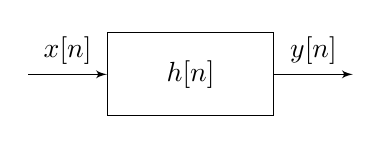
\begin{tikzpicture}[auto,>=latex']
    % We start by placing the blocks
    \node [input, name=input] {};
    \node [block, right=of input] (Impulse) {$h[n]$};
    \node [input, name=output, right=of Impulse] {};
    % We draw an edge between the controller and system block to 
    \draw [->] (Impulse) -- node[name=u] {$y[n]$} (output);
    \draw [->] (input) -- node[name=u] {$x[n]$} (Impulse);
\end{tikzpicture}
\end{figure}

\begin{enumerate}[label=(\alph*)]
  \item Use linearity and shift-invariance properties to show that
\begin{align*}
  y[n]=x[n]*h[n]\stackrel{\Delta}{=}\sum_{k=-\infty}^\infty x[k]h[n-k]=h[n]*x[n].
\end{align*}

This is show that 
\begin{align*}
 \sum_{k=-\infty}^\infty x[k]h[n-k]&\stackrel{?}{=}\sum_{k=-\infty}^\infty h[k]x[n-k]\\
 \sum_{k=-\infty}^\infty x[k]h[n-k]&=\sum_{k=-\infty}^\infty h[n-m]x[m]\text{ \qquad for $m=n-k$, and $k=n-m$}\\
 &=\sum_{n-m=-\infty}^\infty h[m-n]x[m] \text{ \qquad and shifting such that m is an upper bound} \\
 &=\sum^{m=\infty}_{-\infty} h[m-n]x[m] \\
 &\stackrel{\checkmark}{=}\sum_{m=-\infty}^{\infty} h[m-n]x[m] \text{ \qquad which is equivalent under summation}\\
\end{align*}




  \item Define the Fourier transform of a sequence a[n] as 
\begin{align*}
  A(\omega)\stackrel{\Delta}{=}\sum_{n=-\infty}^\infty a[n]e^{-j\omega n}\text{,   } 
-\pi \leq \omega \leq \pi
\end{align*}
and show that the inverse Fourier transform is
\begin{align*}
  a[n]=\frac{1}{2\pi}\int_{-\pi}^\pi A(\omega)e^{+jwn}d\omega\text{,   }-\infty<n<\infty
\end{align*}
I will simply insert the definition of $A(\omega)$ into the inverse FT and solve for $a[n]$
\begin{align*}
  a[n]&=\frac{1}{2\pi}\int_{-\pi}^\pi     \sum_{m=-\infty}^\infty a[m]e^{-j\omega m}             e^{+jwn}d\omega\\
  &=\frac{1}{2\pi}\sum_{m=-\infty}^\infty a[m]     \int_{-\pi}^\pi     e^{-j\omega m}             e^{+jwn}d\omega\\
  &=\frac{1}{2\pi}\sum_{m=-\infty}^\infty a[m]     \int_{-\pi}^\pi     e^{-j\omega (m +n)}d\omega\\
  &=\frac{1}{2\pi}\sum_{m=-\infty}^\infty a[m]         \left[ \frac{e^{j\omega (n-m)}}{j(n-m)}\big|_{-\pi}^\pi\right]\\
  &=\frac{1}{2\pi}\sum_{m=-\infty}^\infty a[m]         \left[ \frac{e^{j\pi (n-m)} -   e^{-j\pi (n-m)}}{j(n-m)}\right]\\
\text{Euler's  }sin(t)=\frac{e^{jt}-e^{-jt}}{2j}\\
  &=\frac{1}{\pi}\sum_{m=-\infty}^\infty a[m]         \frac{sin(\pi(n-m))}{(n-m)}\\
\end{align*}

Here, $sin(\pi(n-m))$ becomes zero for $n\neq m$ as $sin(\pi n)=0$, for $n\in$ integers, 

Finally for $n=m$, $\lim_{n\to 0}\frac{sin(n)}{n}=\pi$

\begin{align*}
  a[m]&=\frac{1}{\pi} a[m]         \frac{sin(\pi(0))}{(0)}\\
  &=\frac{1}{\pi} a[m]         \pi\\
  &\stackrel{\checkmark}{=}a[m] 
\end{align*}





  \item Using the results in (a) and (b), show that
\begin{align*}
  Y(\omega)=H(\omega)X(\omega)\text{,   }-\pi\leq\omega\leq\pi
\end{align*}
for an LSI discrete time system.



\begin{align*}
  Y(\omega)&=H(\omega)X(\omega)\\
  FT\{Y\}(\omega)&=FT\{H\}(\omega)FT\{X\}(\omega)\\
                 &=\sum_{n=-\infty}^\infty h[n]e^{-j\omega n}    \sum_{m=-\infty}^\infty x[m]e^{-j\omega m}\\
                 &=\sum_{n=-\infty}^\infty \sum_{m=-\infty}^\infty h[n]x[m]e^{-j\omega (n + m)}\\
\end{align*}
\begin{align*}
  y[v] &=FT^{-1}\left\{FT\{Y\}(\omega)\right\}\\
  &=FT^{-1}\left\{ \sum_{n=-\infty}^\infty \sum_{m=-\infty}^\infty h[n]x[m]e^{-j\omega (n + m)} \right\}\\
  &=\frac{1}{2\pi}\int_{-\pi}^{\pi}\left\{ \sum_{n=-\infty}^\infty \sum_{m=-\infty}^\infty h[n]x[m]e^{-j\omega (n + m)} \right\}e^{jwv}d\omega \\
  &=\frac{1}{2\pi} \sum_{n=-\infty}^\infty \sum_{m=-\infty}^\infty h[n]x[m]\int_{-\pi}^{\pi}e^{-j\omega (n + m)} e^{jwv}d\omega \\
\end{align*}

And as this is nearly the same integral as before, the only time this isn't zero is at $m+n=v$. At this point, the integral equals $2\pi$.
\begin{align*}
  &=\frac{1}{2\pi} \sum_{n=-\infty}^\infty \sum_{m=-\infty}^\infty h[n]x[m] \pi \\
  &=\sum_{n=-\infty}^\infty  h[n]x[m]\big|_{m=v-n}\\
  &\stackrel{\checkmark}{=}\sum_{n=-\infty}^\infty h[n]x[v-n]\\ 
\end{align*}



\end{enumerate}
\newpage




\section{8.40} 
\subsection{Exercise}
Consider using a first-order Markov sequence to model a random sequence $X[n]$ as 
\begin{align*}
  X[n]=rX[n-1]+Z[n],
\end{align*}
where $Z[n]$ is white noise of variance $\sigma^2_Z$. Thus, we can look at X[n] as the output of passign $Z[n]$ through a linear system. Take $|r|<1$ and assume the system has been running for a long time, that is, $-\infty<n<\infty$




\begin{enumerate}[label=(\alph*)]
 \item Find the psd of $X[n]$, that is, $-\infty<n<\infty$.

White noise implies $\mu_z=0$, $\sigma_Z^2=c$; $c$ constant $\forall n$.

White noise by definition is uncorrelated.  Therefore $E[Z[n]Z[n+l]]=0$ for $l\neq0$, 

From here, the output PSD $S_{XX}$.
\begin{align*}
  S_{XX}(\omega)&=|H(\omega)|^2Z(\omega)\text{, \qquad where $Z(\omega)=\sigma^2_Z$}\\
  &=|H(\omega)|^2\sigma_Z^2
\end{align*}

Start by finding the impulse response.
\begin{align*}
  X[n]&=rX[n-1]+\delta[n]\\
  X[n]-rX[n-1]&=\delta[n]\\
  h[n]-rh[n-1]&=\delta[n]\\
  Z\{h[n]-rh[n-1]\}&=Z\{\delta[n]\}\\
  H(Z)-rZ^{-1}  H(Z)&=1\\
  H(Z)&=\frac{1}{1-rZ^{-1}}\\
\end{align*}

The $FT\{h[n]\}$ is then simply the $Z\{h[n]\}\big|_{Z=e^{-jwn}}$

$H(\omega)=\frac{1}{1-re^{-jwn}}$\\


\begin{align*}
  |H(w)|^2&=\frac{1}{(1-re^{-jwn})(1-re^{-jwn})}\\
  &=\frac{1}{1+(-re^{-jwn})(-re^{-jwn})+2re^{-jwn}}\\
  &=\frac{1}{-re^{-2jwn}+2re^{-jwn}}\\
  &=\frac{1}{1+r^2-2rcos(\omega)}\text{\qquad which I'm still slightly unsure on.}\\
\end{align*}

Finally $S_{XX}=\frac{\sigma^2_Z}{1+r^2-2rcos(\omega)}$


 \item Find the correlation function $R_{XX}[m]$.
\end{enumerate}
\newpage


{\huge This is all I've got at this point. } I will try to complete the rest in the future. I'm really struggling with these homeworks.














\section{8.44} 
\subsection{Exercise}
Given a Markov chain X[n] on $n\geq1$, with the transistion probabilities given as $P\left[x[n]|x[n-1]\right]$, 
find an expression for the two-step transition probabilities $P\left[x[n]|x[n-2]\right]$.
Also show that
\begin{align*}
  P\left[x[n+1]x[n-1],x[n-2],\ldots,x[1]\right]=P\left[x[n+1]x[n-1]\right]\text{,   for } n\geq1.
\end{align*}
\newpage

\section{8.51} 
\subsection{Exercise}
Let $X[n]$ be a real-valued random sequence on $n\geq0$, made up from a stationary and \emph{independent increments}, that is, $X[n]-X[n-1]=W[n]$, ``the increment'' with $W[n]$ being a stationary and independent random sequence. The random sequence always starts
with $X[0]=0$. We also know that at time $n=1$, $E[X[1]]=\nu$ and $Var[X[1]]=\sigma^2$.
\begin{enumerate}[label=(\alph*)]
  \item Fin $\mu_X[n]$ and $\sigma^2_X[n]$, the mean and variance functions of the random 
sequence $X$ at time $n$ for any time $n>1$.
  \item Prove that $\frac{X[n]}{n}$ converges in probability to $\nu$ as the time 
$n$ approaches infinity.
\end{enumerate}
\newpage
\end{document}






